\subsection{Mixture models}
\paragraph{Purpose}
It is the simplest form of \emph{Latent Variable Models (LVMs)} is when $z_{i}\in
\{k\}_{1\leq k\leq K}$. 2 mains application of mixture models:
\begin{itemize}
    \item use them as \emph{black-box} density model, $p(\bm{x}_{i})$, useful for data
        compression, outlier detection and creating generative classifiers
    \item use for clustering
\end{itemize}

\paragraph{Assumptions}
\paragraph{Theory}
We use a discrete prior $p(z_{i}) = \text{\emph{Cat}}(\bm{\pi})$ and the likelihood
$p(\bm{x}_{i}|z_{i} = k)$, finally the \textbf{mixture model} is :
\begin{center}
    $\prob{\bm{x}_{i}|\bm{\theta}} = \su{k=1}{K}\pi_{k}\prob{\bm{x}_{i}|z_{i}=k,
    \bm{\theta}} = \su{k=1}{K}\pi_{k}\mathbb{P}_{k}\left(\bm{x}_{i}|\bm{\theta}\right)$
\end{center}
where $\mathbb{P}_{k}$ is the $k$'th \emph{base distribution}.
\subparagraph{Mixtures of Gaussian}
Each base distribution in the mixture is a multivariate Gaussian with mean $\mu_{k}$ 
and covariance matrix $\bm{\Sigma}_{k}$:
$\prob{\bm{x}_{i}|\bm{\theta}}=\su{k=1}\pi_{k}\mathcal{N}\left(\bm{x}_{i}|\bm{\mu}_{k},
    \bm{\Sigma_{k}}\right)$\\
Given a sufficiently large number of mixture components a \tB{Gaussian Mixture Models
(GMMs) can be used to approximate any density defined on $\mathbb{R}^{D}$}.
\subparagraph{Mixtures of multinoullis}
can be used to define density models on data consisting of a \emph{D}-dimensional bit
vectors: $\prob{\bm{x}_{i}|z_{i}=k,\bm{\theta}} = \prd{j=1}{D}\text{\emph{Ber}}(x_{ij}|
\mu_{jk})=\prd{j=1}{D}\mu_{jk}^{x_{ij}}(1-\mu_{jk})^{1-x_{ij}}$\\
where $\mu_{jk}$ is the probability that bit $j$ turns on in cluster $k$.
\subparagraph{Mixture of experts}
are build from a discriminative perspective, they relies on the idea that a good
model different linear method each applying to a different part of the input space.\\
We can model this by allowing the mixing weights and the mixture densities to be
input-dependent: 
\begin{center}
    $\begin{cases}
        \prob{y_{i}|\bm{x}_{i},z_{i}=k,\bm{\theta}} = \mathcal{N}(y_{i}|\bm{w}_{k}^{T}
        \bm{x}_{i},\sigma_{k}^{2}) \\
        \prob{z_{i}|\bm{x}_{i},\bm{\theta}} = \text{\emph{Cat}}(z_{i}|S(\bm{V}^{T}
        \bm{x}_{i}))
    \end{cases}$
\end{center}
Useful in solving inverse problems, the ones in which we have to invert a many-to-one
mapping, for example in robotics where the location of the end effector (hand) $\bm{y}$
is uniquely determined by the joint angles of the motors, $\bm{x}$.

The overall posterior is then
\begin{center}
    \fr{$\prob{y_{i}|\bm{x}_{i},\bm{\theta}} = \su{k}{}\prob{z_{i}=k|\bm{x}_{i},z_{i}=k
    ,\bm{\theta}}$}
\end{center}




\paragraph{Strengths}

\paragraph{Weaknesses}
\begin{itemize}
    \item Use of a single latent variable to generate the observation
\end{itemize}

\paragraph{Relationships with other methods}
\paragraph{Examples of application}


\subsection{ARD: Automatic Relevance Determination}
\paragraph{Purpose}
To get greater sparsity 
\paragraph{Assumptions}
\paragraph{Theory} 
Relying on empirical bayes, whereby we integrate oute $\bm{w}$ and maximize the 
marginal likelihood $\tau$.
\subparagraph{Linear Regression}
Let's consider weight precisions by $\alpha_{j}=\frac{1}{\tau_{j}^{2}}$ and the 
measurement precision by $\beta=\frac{1}{\sigma^{2}}$:
\begin{center}
    $\begin{cases}
        \prob{y|\bm{x},\bm{w},\beta} = \mathcal{N}\left(y|\bm{w}^{T}\bm{x},\frac{1}{
            \beta}\right) \\
            \prob{\bm{w}} = \mathcal{N}(\bm{w}|0,\bm{A}^{-1})
    \end{cases}$
\end{center}
where $\bm{A}=\text{\emph{diag}}(\bm{\alpha})$
To regularize the problem we may pu a conjugate prior on each precision $\alpha_{j}
\hookrightarrow \text{\emph{Gamma}}(a, b)$ and $\beta \hookrightarrow \text{\emph{
Gamma}}(c, d)$
When performing EB point estimation will use the improper prior $a=b=c=d=0$ which
results in \tB{maximal sparsity}.
\subparagraph{Sparsity}
If $\hat{\alpha}_{j} \approx 0$ we find $\hat{w}_{j}\approx \hat{w}^{mle}_{j}$ since
the Gaussian prior shrinking $w_{j}$ towards 0 has zero precision.\\
However if we find that \uB{$\hat{\alpha}_{j}\rightarrow\infty$ then the prior is very 
confident that $w_{j}=0$ and hence that feature $j$ is "irrelevant"}.
\subparagraph{Logistic Regression}
uses iteratively reweighted $l_{1}$ algorithm.

\paragraph{Strengths}
\paragraph{Weaknesses}
\paragraph{Relationships with other methods}
\paragraph{Examples of application}



\subsection{Sparse coding}
\paragraph{Purpose}
Sparse priors for unsupervised learning, here we relax the constraint that $\bm{W}$
is orthogonal. 
\paragraph{Assumptions}
\paragraph{Theory}
\paragraph{Strengths}
\paragraph{Weaknesses}
\paragraph{Relationships with other methods}
\paragraph{Examples of application}

\subsection{Support Vector Machines (SVMs)}
\paragraph{Purpose}
The \tB{combination of the \emph{kernel trick} plus a modified loss function 
allowing \emph{sparsity}}, meaning that the prediction will only depend on a
subset of the training data called \emph{support vectors}. The overall 
process is known as a \emph{Support Vector Machine}.\\
Because of sparsity encoding in the loss function instead of in the prior, 
kernel encoding through a trick instead of being an explicit part of the 
model,\tB{SVMs do not provide probabilistic outputs}.
\subparagraph{SVMs for regression}
with \emph{kernalized ridge regression} the solution $\bm{w}$ depends on all 
the training inputs. We should then use a variant of \emph{Huber loss} 
function: the \tB{\textit{epsilon insensitive loss function}}: 
\begin{center}
    \fr{$L_{\epsilon}\left(y-\hat{y}\right) = 
    \begin{cases}
        0 & \Leftarrow \lvert y-\hat{y}\rvert < \epsilon \\
        \lvert y-\hat{y}\rvert -\epsilon &\Leftarrow \lvert y-\hat{y}\rvert 
            \geq \epsilon    
    \end{cases}$}
\end{center}
meaning that any point lying inside an $\epsilon\text{-\textbf{tube}}$ a
around the prediction is not penalized: $J=C\su{i=1}{n}L_{\epsilon}\left(
y_{i} - \hat{y}_{i}\right) + \frac{1}{2}\norm{\bm{w}}^{2}$, with $C=\frac{1}{
\lambda}$ is a \emph{regularization constant}.\\
It can be shown that \tB{optimal solution has the form $\hat{\bm{w}} = \su{i}{
}\alpha_{i} \bm{x}_{i}$, where $\alpha_{i}\geq 0$}. It turns out that \tB{
$\bm{\alpha}$ is sparse as we don't care about errors which are smaller than 
$\epsilon$. The $\bm{x}_{i}$ for which $\alpha_{i}>0$ are the \textbf{support 
vectors}}.\\
Then we have $\hat{y}(\bm{x}) = \hat{w}_{0} + \hat{\bm{w}}\bm{x}  = \hat{w}_{0}
+ \su{i}{}\alpha_{i}\bm{x}_{i}^{T}\bm{x} = \su{i}{}\alpha_{i}k(\bm{x},\bm{x}_{i})$

\subparagraph{Classification}
we consider now the \emph{hinge loss}:
\begin{center}
    $L_{hinge}(y,\eta) = \max\left(0, 1-y\eta\right) = \left(1-y\eta\right)_{+}$
\end{center}
where $\eta=f(\bm{x})$ is our 'confidence' in choosing label $y=1$ however it does not
need to have any probabilistic semantics.\\
The overall objective has the form $\min_{\bm{w}:w_{0}}\frac{1}{2}\norm{\bm{w}}^{2} +
C\su{i=1}{n}\left(1-y_{i},f(\bm{x}_{i})\right)$. Same principle as in regression, but
this time \tB{$\hat{y}(\bm{x}) = sgn\left(f(\bm{x})\right) = sgn\left(\hat{w}_{0} +
\hat{\bm{w}}^{T}\bm{x}\right)= sgn\left(\hat{w}_{0} + \su{i=1}{n}\alpha_{i}k(\bm{x}_{i}
,\bm{x})\right)$}
\subparagraph{The large margin principle}
our goal is to derive a \emph{discriminative function} $f(x)$ which will be linear in the feature
space implied by the choice of kernel. Hence: $\bm{x} = \bm{x}_{\perp} + 
r\frac{\bm{x}}{\norm{\bm{w}}}$ where $r$ is the distance of $\bm{x}$ from the decision boundary 
whose normal vector is $\bm{w}$, and $\bm{x}_{\perp}$ is the orthogonal projection of $\bm{x}$a 
onto this boundary. Hence $f(\bm{x}) = \bm{w}^{T}\bm{x} +w_{0} = \left(\bm{x}^{T}\bm{x}_{\perp}
+ w_{0}\right) + r\frac{\bm{w}^{T}\bm{w}}{\norm{\bm{x}}}$. As $f(\bm{x}_{\perp}) = 0$ 
$\bm{w}^{T}\bm{x} +w_{0} = 0$ Hence $f(\bm{x}) = r\frac{\bm{w}^{T}\bm{wl}}{\norm{\bm{x}}}$.
Finally \tB{$r = \frac{f(\bm{x})}{\norm{\bm{x}}}$, the distance that we would like to make as large 
as possible, in order to clearly separate the input}.
\subparagraph{Regularization parameter \emph{C}}
it \tB{controls the number of errors we are willing to tolerate on the training set}, it is chosen by
cross-validation, \uB{an efficient way to chose \emph{C} is to develop a path following algorithm in 
the spirit of \emph{ARS}}.

\paragraph{Assumptions}
\paragraph{Theory}
\paragraph{Strengths}
\begin{itemize}
    \item computational advantages over probabilistic model
    \item \tB{\emph{kernel trick} $\rightarrow$ prevent underfitting}: ensuring that the feature 
        vector is sufficiently rich that a linear classifier can separate
    \item \tB{\emph{sparsity} \& \emph{large margin principles} $\rightarrow$  prevent overfitting}: 
        ensure that we do not use all the basis functions

\end{itemize}

\paragraph{Weaknesses}
\begin{itemize}
    \item issues for multi-class classification due to the non-probabilistic 
        aspect of the model: \uB{output scores are not on a calibrate scale}
\end{itemize}

\paragraph{Relationships with other methods}
\paragraph{Examples of application}

\subsection{MODEL COMPARISON}
\paragraph{Comparison of discriminative kernel methods}
\begin{itemize}
    \item \emph{L1VM}: $l_{1}$-regularized vector machine
    \item \emph{L2VM}: $l_{2}$-regularized vector machine
    \item \emph{SVM}: Support Vector Machine
    \item \emph{RVM}: Relevance Vector Machine
    \item \emph{GP}: Gaussian Process
\end{itemize}
\begin{itemize}
    \item \emph{speed} $\rightarrow$ use RVM
    \item \emph{well-calibrated probabilistic outputs} $\rightarrow$ GP
\end{itemize}
the only circumstances under which using an SVM seems sensible is the structured output
case, where likelihood-based methods can be slow.


\subsection{Gaussian Processes}
\paragraph{Purpose}
It defines a prior over functions, which can be converted into a posterior over 
functions once we have seen some data.\\
They \tB{can be thought of as a Bayesian alternative to the kernel methods}.
\paragraph{Assumptions}
\paragraph{Theory}
\subparagraph{Regression}
Let the prior on the regression function be GP denoted by
$f(\bm{x}) \hookrightarrow \text{\emph{GP}}(m(\bm{x}), k(\bm{x},\bm{x}'))$ where
$m(\bm{x})$ is the mean function and $k(\bm{x}, \bm{x}')$ is the kernel or covariance 
function.
\paragraph{Strengths}
\paragraph{Weaknesses}
\paragraph{Relationships with other methods}
\paragraph{Examples of application}
\begin{itemize}
    \item noise-free GP regression is a computationally cheap proxy for the behavior
        of a complex simulator such as a weather forecasting program.
\end{itemize}




\subsection{Classification And Regression Trees (CART)}
\paragraph{Purpose}
\paragraph{Assumptions}
\paragraph{Theory}
\begin{center}
    $f(\bm{x}) = \E{y|\bm{x}} = \su{m=1}{M}w_{m}\mathbbm{1}_{\{\bm{x}\in R_{m}\}}
\su{m=1}{M}w_{m}\phi(\bm{x};\bm{v}_{m})$
\end{center}
where $R_{m}$ is the m'th region $w_{m}$ is the mean response in this region and 
$\bm{v}_{m}$ encodes the choice of variable to split on.
\subparagraph{Growing a tree}
\begin{center}
    \fr{$(j^{*},t^{*}) = \argmin_{J\in\left\{j\in\inter{1}{D}\right\}} \min_{t\in\mathcal{T}_{
j}} \text{\emph{cost}}(\{\bm{x}_{i},y_{i}:x_{ij}\leq t\}) + \text{\emph{cost}}(
\{\bm{x}_{i},y_{i}:x_{ij}> t\})$}
\end{center}
where the set of possible thresholds $\mathcal{T}_{j}$ for feature $j$ can be obtained
by sorting the unique values of $x_{ij}$
\subparagraph{Cost}
\begin{itemize}
    \item \emph{Regression}: \emph{cost}$(\mathcal{D})=\su{i\in\mathcal{D}}{}\left(
        y_{i}-\overline{y}\right)^{2}$
    \item \emph{Classification}:  knowing that $\hat{\pi}_{c} = \frac{1}{|\mathcal{D}|}
        \su{i\in\mathcal{D}}{}\mathbbm{1}_{\{y_{i}=c\}}$ 
        \begin{itemize}
            \item \emph{Misclassification Rate}: $\frac{1}{|\mathcal{D}|}\su{i\in
                \mathcal{D}}{}\mathbbm{1}_{\{y_{i}\neq\hat{y}\}}$
            \item \emph{Entropy} $\mathbb{H}(\hat{\bm{\pi}}_{c}) =-\su{c=1}{C}\hat{\pi}
                _{c}\log\left(\hat{\pi}_{c}\right)$
            \item \emph{Gini index}: $\su{c=1}{C}\hat{\pi}_{c} (1-\hat{\pi}_{c})$, 
        \end{itemize}
\end{itemize}
Cross-entropy and Gini measures are very similar and more sensitive to changes in class
probability than is the misclassification rate, finally they favor \emph{pure nodes}
\subparagraph{Pruning}
As stopping growing the tree to prevent overfitting would provoke to miss making any
splits because of feature on its own has little predictive power.\\
\uB{Growing a "full" tree then performing \emph{pruning} is better}.
\subparagraph{Random Forest}
\tB{to reduce the variance of an estimate, we can train M different trees on
different subsets of the data}, randomly chosen with replacement and compute:
\begin{center}
    $f(\bm{x}) = \su{m=1}{M}\dfrac{1}{M}f_{m}(\bm{x})$
\end{center}
where $f_{m}$ is the \emph{m}'th tree. This called \tB{\textbf{bagging (bootstrap 
aggregating)}}\\
Simply re-running the sample learning algorithm on different subsets of the data can
result in highly correlated predictors.\\
\tB{The \textbf{random forest} technique tries to decorrelate the base learners by 
learning trees based on a randomly chosen subset of input variables as well as a
randomly chosen subset of data cases} (observations). 




 


\paragraph{Strengths}
\begin{itemize}
    \item easy to interpret
    \item handle mixed discrete and continuous input
    \item insensitive to monotone transformation of the inputs (because the splits
        are based on ranking the data points)
    \item automatic variable selection 
    \item relatively robust to outliers
    \item scale well to large datasets
    \item can be modified to handle missing inputs
\end{itemize}


\paragraph{Weaknesses}
\begin{itemize}
    \item less accurate that other kinds of model (partly due to the greedy nature of
        the tree construction)
    \item unstable: small changes to the input data can have large effect on the 
        structure of the tree (due to hierarchical nature of the tree-growing process)
    \item causing errors at the top can affect the rest of the tree
\end{itemize}

\paragraph{Relationships with other methods}
\paragraph{Examples of application}

\subsection{Generalized Additive models}
\paragraph{Purpose}
To create a nonlinear model with multiple inputs: $f(\bm{x}) = \alpha + \su{i=1}{D}f_{
i}(x_{i})$
\paragraph{Assumptions}
\paragraph{Theory}
The loss function in regression setting:
$J\left(\alpha,(f_{i})_{1\leq i\leq D}\right) = \su{i=1}{n}\left(y_{i}-\alpha -
\su{j=1}{D}f_{i}(x_{ij})\right)^{2} + \su{j=1}{D}\lambda_{j}\Su{}{}f_{j}^{''}(t_{j})^{
2}dt_{j}$ where $\lambda_{j}$ is the strength of the regularizer for $f_{j}$
\subparagraph{Multivariate Adaptive Regression Splines (MARS)}
We create an ANOVA decomposition:
$f(\bm{x}) = \beta_{0} + \su{j=1}{D}f_{j}(x_{j}) + \su{j,k}{}f_{jk}(x_{j},x_{k}) + 
\su{j,k,l}{}f_{j,k,l}(x_{j}, x_{k}, x_{l}) + \cdots$
\paragraph{Strengths}
\paragraph{Weaknesses}
\paragraph{Relationships with other methods}
\paragraph{Examples of application}

\subsection{Boosting}
\paragraph{Purpose}
It is a greedy algorithm for fitting adaptive basis-function models \tB{$f(\bm{x}) = 
w_{0} + \su{m=1}{M}w_{m}\phi_{m}(\bm{x})$}, where $\phi_{m}$ are generated by an
algorithm called \textbf{weak learner}. \uB{This algorithm works by applying the weak
learner sequentially to weighted versions of the data, where more weight is given to
examples that were misclassified by earlier rounds.}\\
This weak learner can be any classification or regression algorithm, but \tB{it common
to use CART model}.\\
\tB{Boosting is very resistant to overfitting.}\\
\subparagraph{Forward stagewise additive modeling}
The goal of boosting is to solve the following optimization problem:
\begin{center}
    $\min_{f}\su{i=1}{n}L(y_{i},f(\bm{x}_{i}))$
\end{center}
$f^{*}(\bm{x}) = \argmin_{f(\bm{x})}$

\begin{enumerate}
    \item initialise by defining $f_{0}(\bm{x}) = \argmin_{\gamma}\su{i=1}{n}L\left(
        y_{i},f(\bm{x};\gamma)\right)$, for example if we use squared error we can
        set $f_{0}(\bm{x})=\overline{y}$
    \item at iteration $m$ we compute $(\beta_{m},\gamma_{m}) = \argmin_{\beta,\gamma}
        \su{i=1}{n}L\left(y_{i},f_{m-1}(\bm{x}_{i})+\beta\phi(\bm{x}_{i};\gamma)
        \right)$
    \item $f_{m}(\bm{x}) = f_{m-1}(\bm{x}) + \beta_{m}\phi_{m}(\bm{x}_{i};\gamma)$
\end{enumerate}

\begin{center}
    \begin{tabular}{|*{5}{c|}}
    \hline
    \textbf{Name} & \textbf{Loss}& \textbf{Derivate}& \textbf{$f{*}$} & \textbf{Algorithm}\\
    \hline
    \emph{Squared error} & $\frac{1}{2}\left(y_{i}-f(\bm{x}_{i})\right)^{2}$ & 
    $y_{i}-f(\bm{x}_{i})$ & $\E{y|\bm{x}_{i}}$ & \emph{L2Boosting}\\
    \hline
    \emph{Absolute error} & $|y_{i}-f(\bm{x}_{i}|$ & 
    $sgn(y_{i}-f(\bm{x}_{i}))$ & \emph{median}$(y|\bm{x}_{i})$ & \emph{Gradient 
    Boosting}\\
    \hline
    \emph{Exponential loss} & $\exp\left(-y_{i},f(\bm{x}_{i})\right)$ & $-y_{i}\exp(
    -y_{i}f(\bm{x}_{i}))$ & $\frac{1}{2}\log\left(\frac{\pi_{i}}{1 - \pi_{i}}\right)$&
    \emph{AdaBoost}\\
    \hline
    \emph{Logloss} & $\log\left(1+e^{-y_{i}f(\bm{x}_{i})}\right)$ & $-y_{i}-\pi_{i}$ &
    $\frac{1}{2}\log\left(\frac{\pi_{i}}{1 - \pi_{i}}\right)$ & \emph{LogitBoost}\\
    \hline
    \end{tabular}
\end{center}
where $\pi=\sigma\left(2f(\bm{x})\right)$


\paragraph{Assumptions}
\paragraph{Theory}
\paragraph{Strengths}
\paragraph{Weaknesses}
\paragraph{Relationships with other methods}
\paragraph{Examples of application}

\subsection{Ensemble learning}
\paragraph{Purpose}
Refers to learning a weighted combination of base models of the form:
$f(y|\bm{x},\bm{\pi}) = \su{m\in\mathcal{M}}{}w_{m}f_{m}(y|\bm{x})$ where $w_{m}$ are
the tunable parameters.
\paragraph{Assumptions}
\paragraph{Theory}
\subparagraph{Stacking}
To estimate the weights we can use : $\hat{\bm{w}} = \displaystyle\argmin_{\bm{
w}}\su{i=1}{n}L\left(y_{i},\su{m=1}{M}w_{m}\hat{f}_{m}^{-i}(\bm{x})\right)$, with 
$\hat{f}_{m}^{-i}(\bm{x}$ being the predictor obtained by training on data excluding
$(\bm{x}_{i},y_{i})$. It would allow to avoid overfitting that would produce in using
simply $f_{m}$. This know as \textbf{stacking}.
\paragraph{Strengths}
\paragraph{Weaknesses}
\paragraph{Relationships with other methods}
\paragraph{Examples of application}
\begin{itemize}
    \item analogy with neural networks: $f_{m}$ representing the $m^{th}$ hidden unit 
        and $w_{m}$ are the outputs layer weights
    \item analogy with boosting: where the weights on the base models are determined 
        sequentially
\end{itemize}


\subsection{Multi-layer Perceptron}
\paragraph{Purpose}
It is a \tB{series of logistic regression models stacked on top of each other}, with the final layer
being another logistic regression or a linear regression model.

\paragraph{Assumptions}
\paragraph{Theory}
For a three layers regression problem the model has the form:
$\begin{cases}
    \prob{y|\bm{x},\bm{\theta}} &= \mathcal{N}\left(y|\bm{w}^{T}\bm{z}(\bm{x}), \sigma^{2}\right)\\
    \bm{z}(\bm{x}) &= g(\bm{V}\bm{x})
\end{cases}$
where \tB{$g$ is a non-linear activation function} (usually the logistic function), \uB{$\bm{V}$ is 
the weight matrix from the input to the hidden nodes} and \uB{$\bm{w}$ is the weight vector from 
hidden nodes to the output}.
\begin{figure}[H]
    \begin{center}
        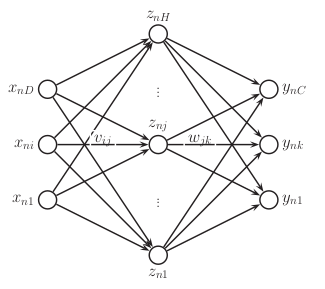
\includegraphics[width=.5\textwidth]{./chapters/3_classical_learning/01_supervised_learning/3_images/1_neural_network_one_hl.png}
    \end{center}
    \caption{caption}
    \label{fig:1_neural_network_one_hl}
\end{figure}
\subparagraph{Convolutional Neural Networks}
It is an MLP in which \tB{the hidden units have local receptive fields}, and in which \tB{the weights
are \emph{tied} or \emph{shared} across the image in order to reduce the number of parameters}. 
Intuitively the \tB{effect of such spatial parameter tying is that any useful features that are 
"discovered" in some portion of the image can be re-used everywhere else without having to be
independently learned}. The resulting network then exhibits \emph{translation invariance} meaning
it can classify patterns no matter where they occur inside the input image.

\paragraph{Strengths}
\paragraph{Weaknesses}
\paragraph{Relationships with other methods}
\paragraph{Examples of application}


%\subsection{Logistic Regression}
%\paragraph{Purpose}
%\paragraph{Assumptions}
%\paragraph{Theory}
%\paragraph{Strengths}
%\paragraph{Weaknesses}
%\paragraph{Relationships with other methods}
%\paragraph{Examples of application}
